% vim: set textwidth=78 autoindent:

\section{Dxf2Shape Konverter Plugin}\index{Plugins!DXF2Shape Konverter}

% when the revision of a chapter has been finalized, 
% comment out the following line:
%\updatedisclaimer

Das Plugin \toolbtntwo{dxf2shp_converter}{Dxf2Shape Konverter} erm�glicht es,
Vektorlayer von DXF (Drawing Interchange Format) ins Shape-Format zu
konvertieren. Dazu m�ssen Sie folgende Parameter angegeben:

\begin{itemize}
\item \textbf{DXF-Eingabedatei}: Geben Sie hier den Pfad zur DXF-Datei an.
\item \textbf{Ausgabedatei}: Geben Sie hier einen Namen f�r das Ausgabe-Shape
an.
\item \textbf{Typ der Ausgabedatei}: Geben Sie hier den Geometrietyp an.
Unterst�tzt wird momentan Polylinie, Polygon oder Punkt.
\item \textbf{Beschriftungen exportieren}: Wenn Sie dieses Kontrollk�stchen
aktivieren, wird ein zus�tzlicher Shapefile Punktlayer erstellt, und die
damit verkn�pfte dbf-Datei enth�lt die Beschriftungen und Informationen dazu,
die sich im "'TEXT"'-Feld der Datei befinden.
\end{itemize}

\begin{figure}[ht]
   \begin{center}
   \caption{Dxf2Shape Konverter Plugin \nixcaption}\label{fig:dxf2shape_dialog}\smallskip
   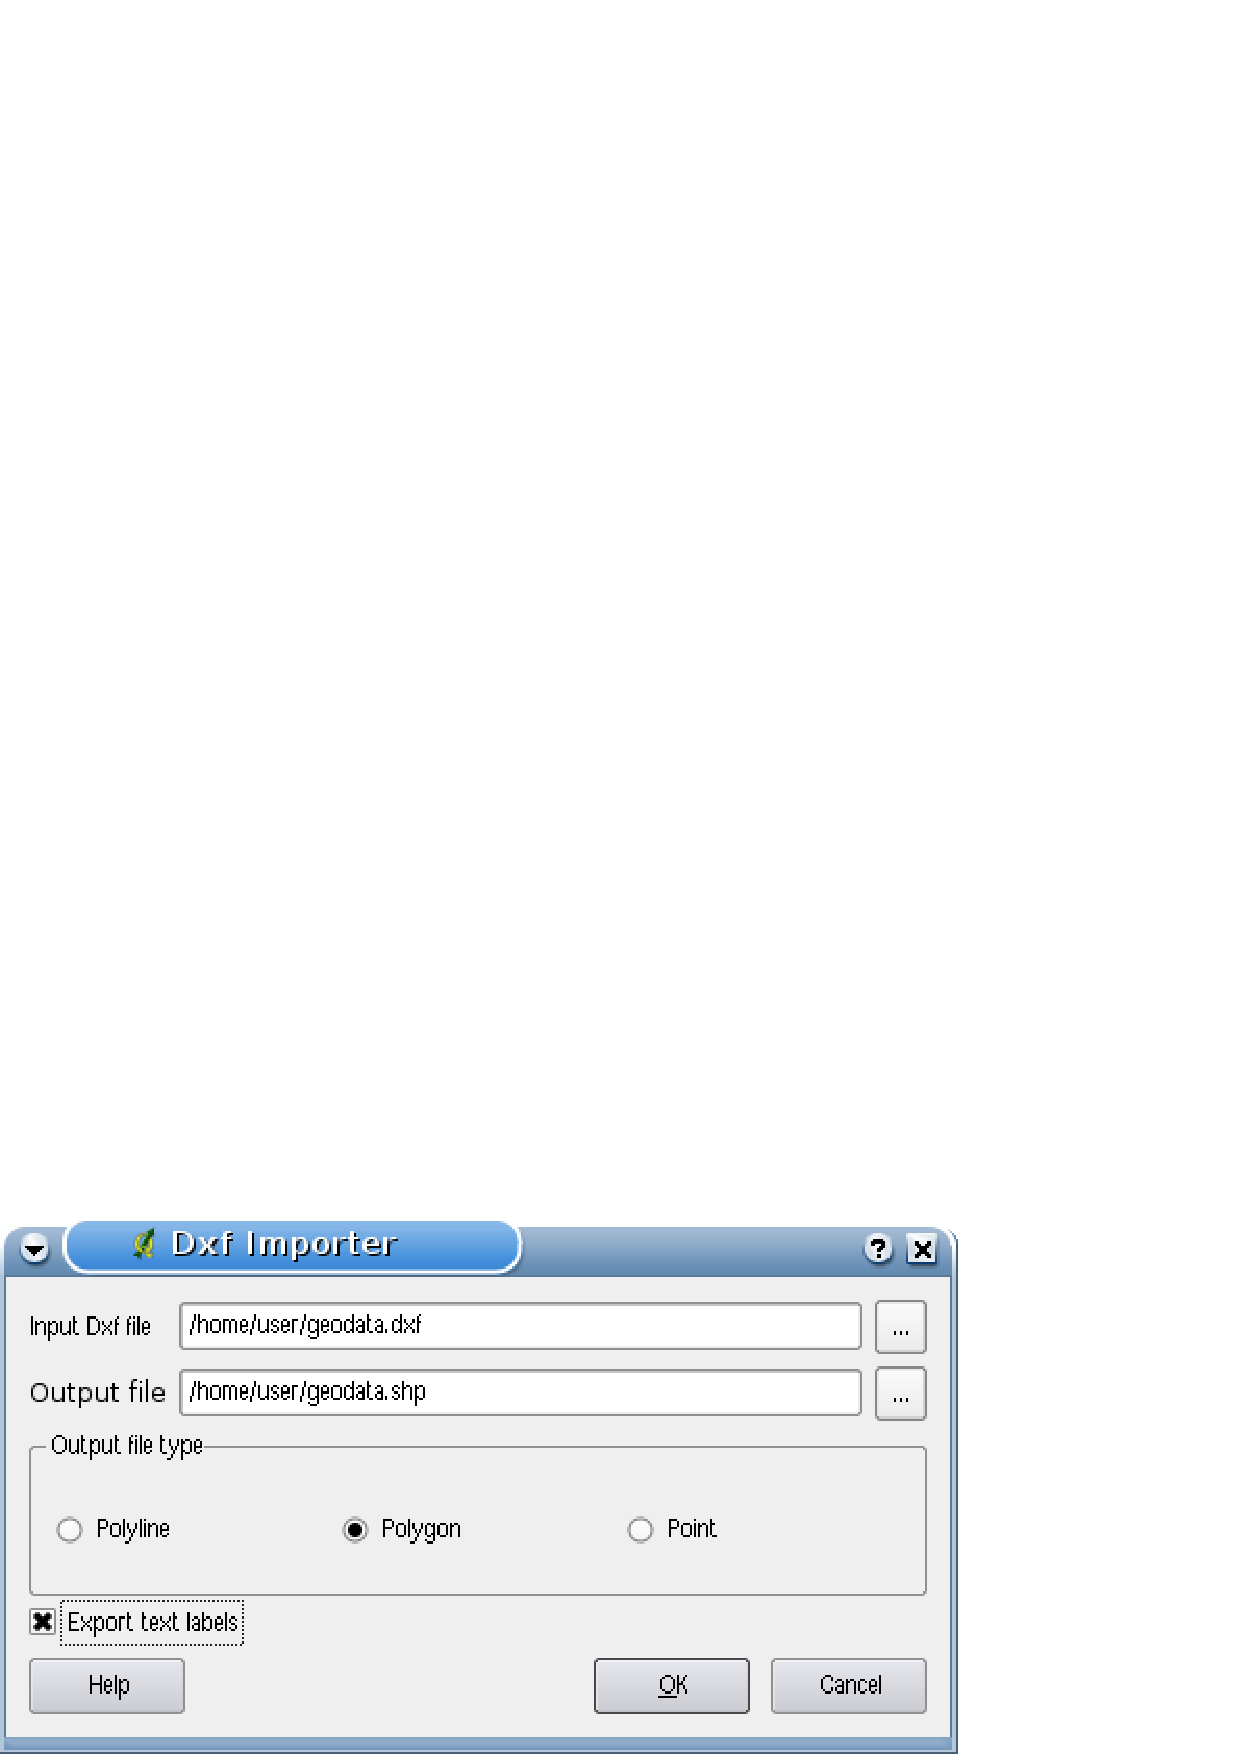
\includegraphics[clip=true, width=10cm]{dxf2shape_dialog}
\end{center}  
\end{figure}

\minisec{Das Plugin anwenden}

\begin{enumerate}
  \item Starten Sie QGIS, laden Sie das Dxf2Shape Plugin mit dem Plugin
Manager (siehe Kapitel~\ref{sec:load_core_plugin}) und klicken Sie auf das
Icon \toolbtntwo{dxf2shp_converter}{Dxf2Shape Konverter} in der
Wekrzeugleiste. Der \dialog{DXF-Import} Dialog erscheint wie in
Abbildung~\ref{fig:dxf2shape_dialog}.
  \item Geben Sie den DXF-Eingabedatei an, einen Namen f�r die Ausgabedatei
und ihren Typ.
  \item Aktivieren Sie das Kontrollk�stchen \checkbox{Beschriftungen
exportieren}, wenn Sie einen zus�tzlichen Shapefile Punktlayer mit den
Beschriftungen erstellen wollen.
  \item Klicken Sie \button{Ok}. 
\end{enumerate}

\newpage

